\newpage{\pagestyle{empty}\cleardoublepage}
\newpage
\vspace*{\fill}
    \begin{center}
      \thispagestyle{empty} \vspace*{0cm} \textbf{\huge
Dise\~{n}o}
    \end{center}
    \vspace*{\fill}
\newpage{\pagestyle{empty}\cleardoublepage}
\chapter{Modelo Entidad Relaci\'{o}n}

Debido al tama\~{n}o del diagrama generado se ha procedido a mostrarlo por partes, de forma que se pueda ver con mayor detalle todo el modelo.

\section{Atributos y entidades}
\begin{figure}[h!]
\centering
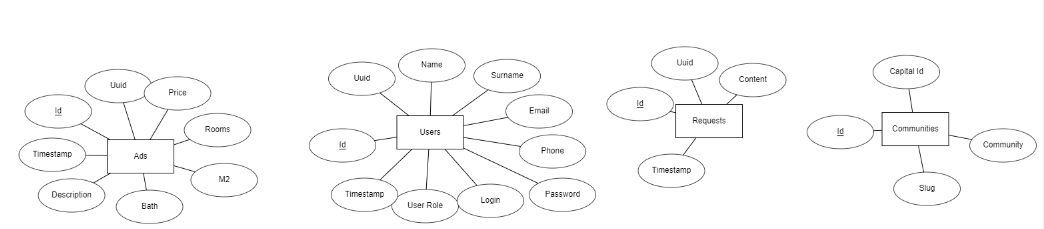
\includegraphics[width=1\textwidth]{Img/Disenyo/ER/upohouse_er_attr_1.PNG}
\end{figure}
\begin{figure}[h!]
\centering
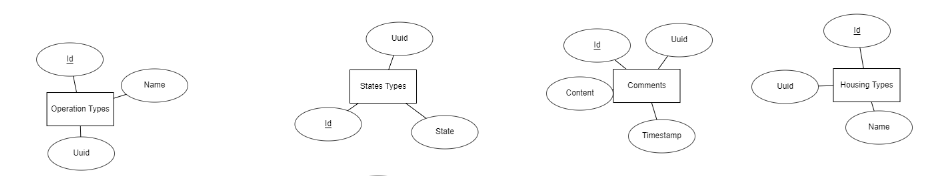
\includegraphics[width=1\textwidth]{Img/Disenyo/ER/upohouse_er_attr_2.PNG}
\end{figure}
\begin{figure}[h!]
\centering
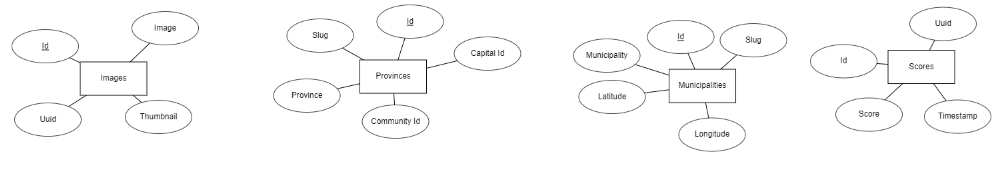
\includegraphics[width=1\textwidth]{Img/Disenyo/ER/upohouse_er_attr_3.PNG}
\end{figure}

\pagebreak

\begin{figure}[h!]
\centering
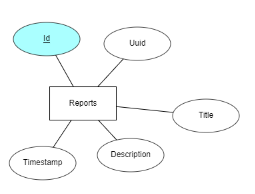
\includegraphics[width=.4\textwidth]{Img/Disenyo/ER/upohouse_er_attr_4.PNG}
\label{fig:dcu}
\end{figure}



\section{Relaciones y entidades}
\begin{figure}[h!]
\centering
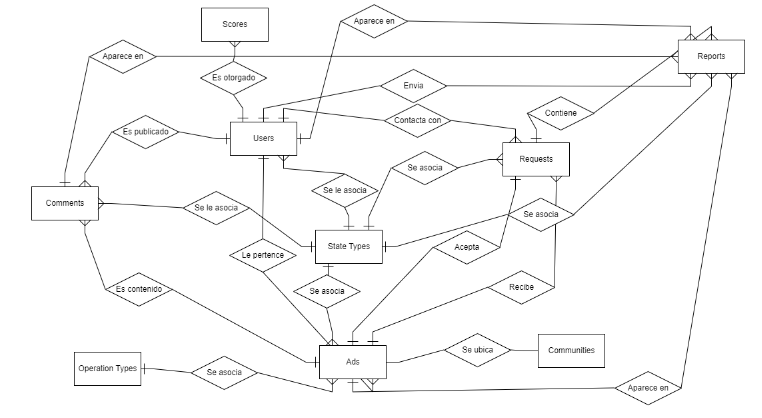
\includegraphics[width=1\textwidth]{Img/Disenyo/ER/upohouse_er_rel_1.PNG}
\label{fig:dcu}
\end{figure}

\begin{figure}[h!]
\centering
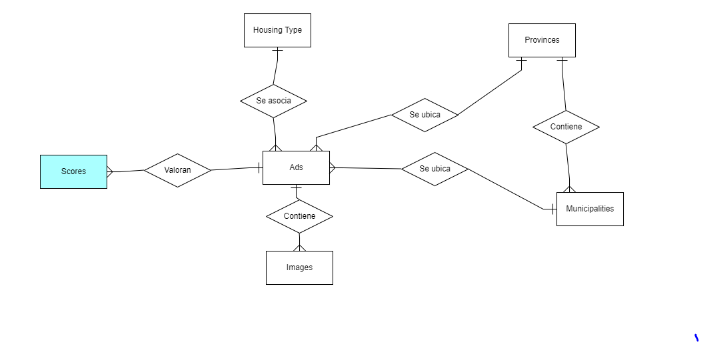
\includegraphics[width=1\textwidth]{Img/Disenyo/ER/upohouse_er_rel_2.PNG}
\label{fig:dcu}
\end{figure}